\chapter{Implementation} 

%%%%%%%%%%%%%%%%%%%%%%%%%%%%% Introduction %%%%%%%%%%%%%%%%%%%%%%%%%%%%%

\section*{Introduction}

This chapter describes the implementation details of the Collaborative Highway Surveillance (CHS) system developed for real-time detection of speeding violations. It presents the tools, libraries, and development environments used to build, integrate, and test the communication modules, routing logic, and prediction components. Special attention is given to the configuration and synchronization of UAVs and ground nodes, ensuring stable data exchange and minimal latency across the network.

Next, we detail the development of the communication protocol, combining MAVLink for drone-to-drone and drone-to-ground communication with UDP for lightweight sensor data transmission. The distributed drone selection algorithm is implemented to account for residual energy, proximity to target zones, and avoidance of redundant coverage.

We then describe the integration of the machine learning prediction module, trained on historical and simulated speeding data to anticipate infraction hotspots. The implementation ensures that computationally heavy operations are executed on ground stations when possible, preserving UAV autonomy.

The final section focuses on system optimization, including strategies for reducing energy consumption, improving communication reliability, and achieving a balance between real-time responsiveness, processing requirements, and operational scalability.

%%%%%%%%%%%%%%%%%%%%%%%%%%%%% Problematic and Objectives %%%%%%%%%%%%%%%%%%%%%%%%%%%%%

\section{Choice of Physical Material}

Before selecting drones for experimentation, it is crucial to clearly define the operational requirements. 
Deploying a drone-based surveillance infrastructure requires consideration of both technical and 
regulatory constraints associated with the equipment. In order to choose suitable drones, several 
selection criteria were evaluated as presented in Table~\ref{tab:drone_criteria}.

\begin{table}[H]
\centering
\caption{Drone selection criteria}
\label{tab:drone_criteria}
\begin{tabular}{|p{4cm}|p{9cm}|}
\hline
\textbf{Criteria} & \textbf{Details} \\ \hline
Flight capabilities & Endurance, maximum speed, transmission range \\ \hline
Camera specifications & Resolution, low-light performance, overall image quality \\ \hline
Technical aspects & Ease of integration into the communication network, 
synchronization with protocols, compatibility with detection and obstacle-avoidance systems \\ \hline
Regulatory aspects & Compliance with national aviation regulations and safety standards, 
respect for privacy and data protection (e.g., EU directives) \\ \hline
Performance and reliability & User feedback, stability of performance, low maintenance requirements \\ \hline
Cost and budget & Operational expenses, financing options, availability of subsidies \\ \hline
Support and services & Availability of technical support, after-sales service, spare parts and repair facilities \\ \hline
Sustainability & Low environmental impact, long-term operational viability \\ \hline
\end{tabular}
\end{table}

Based on these requirements, three categories of drones were identified as particularly relevant:  
\begin{itemize}
    \item \textbf{Pixhawk/Ardupilot-based drones}: Open-source, modular, and programmable platforms, adaptable to mission needs.  
    \item \textbf{DJI Inspire 2}: Professional-grade, robust, and reliable in challenging environments.  
    \item \textbf{Holybro X500 V2 and Hexsoon EDU 450}: Highly flexible, supported by an active open-source community.  
\end{itemize}

\begin{figure}[H]  
    \centering
    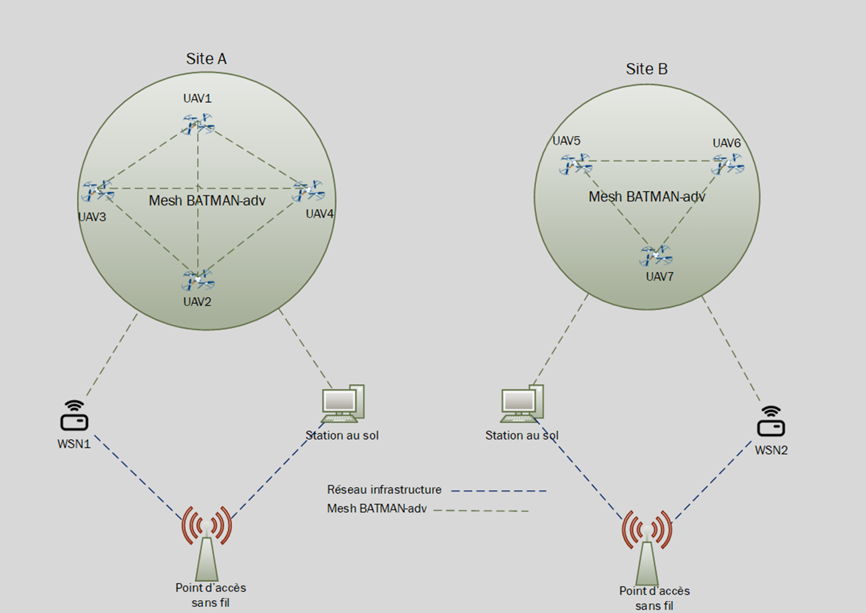
\includegraphics[width=1.0\textwidth]{Figures/Chapter5/Section2/archi.png} % Adjust width as needed
    \caption{Proposed CHS system architecture.}
    \label{fig:proposed_architecture} % Reference label
\end{figure}


The selection of drones for highway surveillance must therefore be guided by operational needs, 
technical and regulatory constraints, as well as economic and environmental considerations.  
Figure~\ref{fig:chs_architecture} illustrates the proposed system architecture.

\subsection*{Selection of Equipment}

The choice of supporting hardware was made according to both technical and financial constraints. 
Performance, reliability, and adaptability were identified as key criteria, which led us to select 
Pixhawk-based drones with the Ardupilot firmware.

\subsubsection*{Pixhawk-based Drones}

The Pixhawk 2.4.8 flight controller (Figure~\ref{fig:pixhawk}) was selected due to its high modularity.  
Pixhawk-based drones allow extensive hardware and software customization, making them suitable 
for this project. They are compatible with a wide range of sensors, communication modules, and 
navigation tools, enabling specific mission configurations while ensuring the desired performance.  
Pixhawk is an open-source flight controller developed by PX4 and supports both PX4 and Ardupilot 
autopilot software.

\begin{figure}[H]  
    \centering
    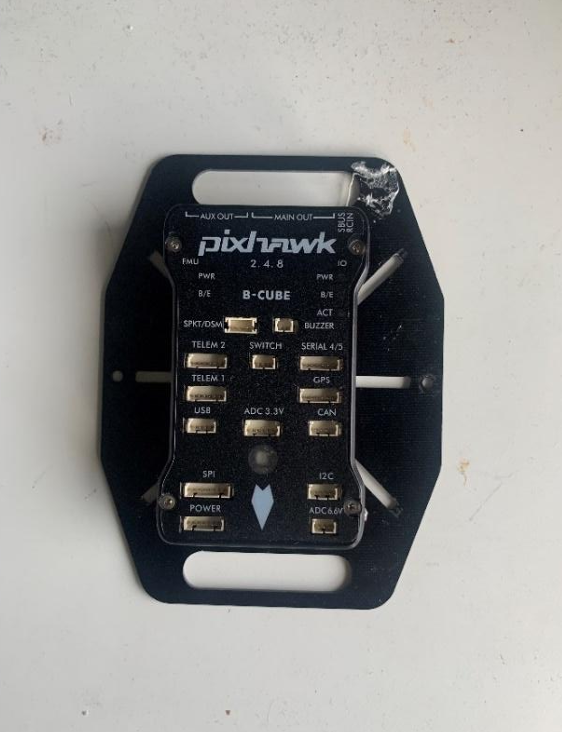
\includegraphics[width=0.5\textwidth]{Figures/Chapter5/Section2/pixhawk.png} % Adjust width as needed
    \caption{Proposed CHS system architecture.}
    \label{fig:proposed_architecture} % Reference label
\end{figure}


For the drone frames, we selected the \textbf{DJI F450} and \textbf{Turnigy SK450} (Figure~\ref{fig:frames}), 
equipped with the flight controller and necessary accessories to achieve autonomous flight.  
The complete hardware setup includes:  

\begin{itemize}
    \item Pixhawk PX4 2.4.8 flight controller  
    \item Ublox NEO-M8N GPS module for navigation and autonomy  
    \item 2212 920KV 30A brushless motors (2 CW, 2 CCW)  
    \item Multistar 20A ESCs (x4)  
    \item Propellers: 2 CW, 2 CCW  
    \item F450 frame: 450mm width, 55mm height, 280g (395g with accessories)  
    \item Raspberry Pi Zero 2 W for telemetry and mesh networking, also equipped with a camera  
    \item Raspberry Pi Camera module  
    \item Power Distribution Board (PDB) to manage power delivery and supply the Raspberry Pi  
    \item MicroSD card for flight data and system logs  
    \item LiPo batteries (Zeee 3S 2200mAh 11.1V 50C or 5200mAh 80C)  
    \item LiPo charger  
    \item Power module for battery monitoring by the flight controller  
\end{itemize}

\subsubsection*{Raspberry Pi Zero 2 W}

The Raspberry Pi Zero 2 W (Figure~\ref{fig:rpi}) is a single-board computer running Linux, 
widely used in IoT and embedded applications. With integrated Wi-Fi (2.4GHz) and Bluetooth 4.2, 
it can communicate with other devices in a network. Its GPIO pins support extensions such as sensors 
and modules, making it suitable for telemetry and onboard image capture in our drone setup.  

Its main specifications are:  
\begin{itemize}
    \item Broadcom BCM2710A1, quad-core Cortex-A53 64-bit 1GHz CPU  
    \item 512 MB LPDDR2 SDRAM  
    \item 2.4GHz 802.11 b/g/n Wi-Fi  
    \item Bluetooth 4.2 / BLE, integrated antenna  
    \item Mini HDMI, micro USB OTG  
    \item MicroSD card slot  
    \item CSI-2 camera connector  
    \item 40-pin GPIO header footprint  
    \item Micro USB power supply  
    \item Composite video and reset pins via test pads  
    \item H.264/MPEG-4 decoding (1080p30), H.264 encoding (1080p30)  
\end{itemize}

\begin{figure}[H]  
    \centering
    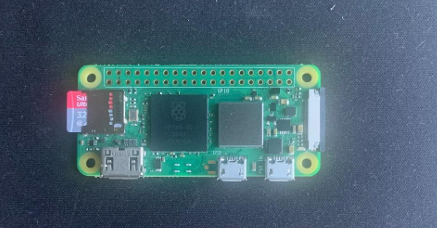
\includegraphics[width=0.5\textwidth]{Figures/Chapter5/Section2/pi2w.png} % Adjust width as needed
    \caption{Proposed CHS system architecture.}
    \label{fig:proposed_architecture} % Reference label
\end{figure}

\begin{figure}[H]  
    \centering
    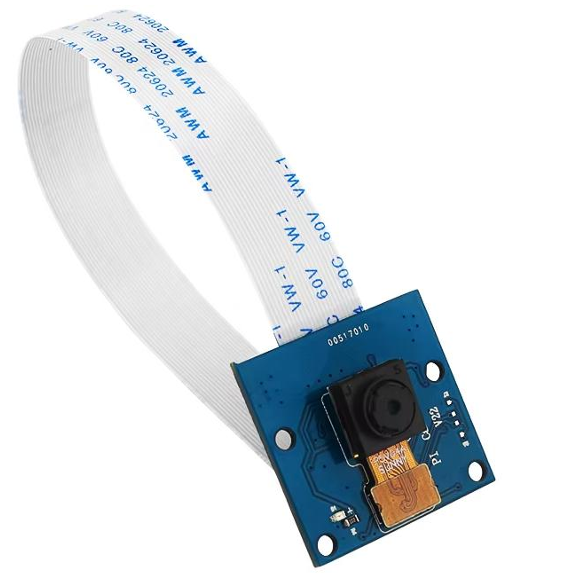
\includegraphics[width=0.5\textwidth]{Figures/Chapter5/Section2/camera.png} % Adjust width as needed
    \caption{Proposed CHS system architecture.}
    \label{fig:proposed_architecture} % Reference label
\end{figure}

\section{Choice of Tools and Development Environment}

The implementation of the Collaborative Highway Surveillance (CHS) system required a 
combination of programming languages, development tools, communication protocols, 
and machine learning frameworks. This section presents the main tools and environments 
used during the development process.

\subsection*{Programming Language}
The majority of the implementation was carried out in \textbf{Python}. This language was chosen 
for its flexibility, extensive libraries, and compatibility with both the Raspberry Pi and 
drone communication frameworks. Python was used to implement the communication 
protocols (UDP and MAVLink), the distributed decision-making algorithm, and 
the integration of computer vision and machine learning modules. 

\subsection*{Communication and Drone Control}
\begin{itemize}
    \item \textbf{MAVLink (Micro Air Vehicle Link)}: a lightweight messaging protocol 
    widely used in unmanned aerial systems for communication between drones, sensors, 
    and ground stations.  
    \item \textbf{PyMAVLink}: the Python implementation of MAVLink, used to encode and 
    decode messages exchanged in the system.  
    \item \textbf{UDP sockets}: implemented to support direct communication between 
    drones and ground nodes (RN/NH).  
    \item \textbf{Crazyflie Python API and Crazyradio}: employed during early testing 
    with Crazyflie drones before integration with Pixhawk-based platforms.  
\end{itemize}

\subsection*{Firmware and Flight Control}
The drones were equipped with the \textbf{Pixhawk 2.4.8 flight controller} running 
the \textbf{Ardupilot} firmware. Ardupilot was selected for its open-source nature, 
flexibility, and wide community support. It allowed the configuration of autonomous 
flight missions while ensuring compatibility with MAVLink. PX4 was also considered, 
but Ardupilot was retained as the primary firmware for this project.

\subsection*{Onboard Processing Environment}
For onboard processing, the \textbf{Raspberry Pi Zero 2 W} was integrated with the drones. 
This single-board computer ran \textbf{Raspberry Pi OS (Linux-based)} and hosted the 
Python scripts responsible for telemetry, communication with ground sensors, 
and computer vision tasks. Its Wi-Fi connectivity was used to establish a mesh 
network between drones.

\subsection*{Ground Control Software}
Two Ground Control Station (GCS) applications were used:  
\begin{itemize}
    \item \textbf{Mission Planner}: mainly for configuring Ardupilot parameters, 
    uploading missions, and monitoring telemetry.  
    \item \textbf{QGroundControl}: used as an alternative interface for visualization 
    and debugging of flight data.  
\end{itemize}

\subsection*{Machine Learning Tools}
Machine learning algorithms for predicting speed violations were developed 
using the following tools:  
\begin{itemize}
    \item \textbf{Scikit-learn}: for preprocessing, feature extraction, and classical ML algorithms 
    such as regression and classification.  
    \item \textbf{TensorFlow/PyTorch}: considered for advanced training tasks and 
    neural networks, particularly for handling more complex datasets.  
    \item \textbf{Jupyter Notebook}: used for prototyping, training, and analyzing 
    machine learning models.  
\end{itemize}

\subsection*{Computer Vision Tools}
To detect and validate speed violations using drone cameras, computer vision 
techniques were implemented with:  
\begin{itemize}
    \item \textbf{OpenCV}: for image preprocessing, frame extraction, and speed estimation 
    through motion analysis.  
    \item \textbf{YOLO (You Only Look Once)}: for real-time object detection and vehicle recognition, 
    enabling the system to detect vehicles directly from the drone’s onboard camera feed.  
    \item \textbf{Raspberry Pi Camera API}: for integrating the onboard camera with the 
    Raspberry Pi module.  
\end{itemize}

\subsection*{Collaboration and Documentation Tools}
For project management and documentation:  
\begin{itemize}
    \item \textbf{Git and GitHub}: for version control and collaborative development.  
    \item \textbf{LaTeX}: for the preparation and formatting of the thesis document.  
\end{itemize}


\section{Communication Protocol Implementation}





\section{Distributed Decision Algorithm}

This section details the mission--to--UAV assignment strategy implemented to guarantee
(i) one UAV per hotspot/mission at any time, (ii) safe battery-aware operations, and
(iii) opportunistic deployment toward likely infraction zones when no real missions are pending.
The method is formulated as a search over a discrete decision tree and solved using a
beam search guided by a distance--priority heuristic. The implementation is provided in
\texttt{algorithm.py} and integrates tightly with the system database (SQLAlchemy models
\texttt{UAV}, \texttt{UAVStatus}, \texttt{Mission}, \texttt{WSN}).

\subsection*{Design Goals and Assumptions}
\begin{itemize}
  \item \textbf{Goal}: select a set of UAV--mission pairs that maximizes an operational score
        (high-priority missions, short travel), while respecting energy constraints and ensuring
        uniqueness (one UAV per mission, one UAV per hotspot).
  \item \textbf{Inputs}: the latest UAV states (position, battery, status), the list of pending missions
        (each bound to a WSN location and a priority), and a probability map over WSNs that do not
        yet have missions (potential hotspots).
  \item \textbf{Outputs}: a mapping \(\mathcal{A}: \text{MissionID} \rightarrow \text{UAV}\), the search trace
        (graph on disk), and logs for auditability.
  \item \textbf{Single-shot planning}: assignments are computed for the current planning window
        (re-planning can be triggered periodically by the scheduler).
\end{itemize}

\subsection*{Decision-Making Architecture}
The software architecture follows four layers:
\begin{enumerate}
  \item \textbf{Data layer} (SQLAlchemy): fetches UAVs, most recent \texttt{UAVStatus}, pending
        \texttt{Mission}s, and all \texttt{WSN}s.
  \item \textbf{Preprocessing layer}: (i) enforces minimum mission priority of 1; (ii) promotes UAVs
        from \texttt{off} to \texttt{standby} if battery \(\geq\) \texttt{MIN\_BATTERY\_FOR\_STANDBY}; (iii)
        builds a WSN probability map for potential hotspots.
  \item \textbf{Search layer}: constructs and explores a decision tree whose nodes (\texttt{SystemStateNode})
        encode multi-UAV system states; exploration uses \emph{beam search}.
  \item \textbf{Reporting layer}: saves a textual trace (\texttt{decision\_graph.txt}) and a colored
        Graphviz PNG (\texttt{decision\_graph.png}) highlighting the best path.
\end{enumerate}

\subsection*{State Space and Constraints}
Each search node \(s\) captures the multi-agent state:
\[
s = \Big(\underbrace{\texttt{uav\_states}}_{\text{positions \& batteries}},
           \underbrace{\texttt{assignments}}_{\text{Mission}\rightarrow\text{UAV}},
           \underbrace{\texttt{path}}_{\text{sequence of (UAV,target)}},
           \texttt{score}, \texttt{depth},
           \underbrace{\texttt{remaining\_missions}}_{\mathcal{M}},
           \underbrace{\texttt{remaining\_uavs}}_{\mathcal{U}},
           \underbrace{\texttt{remaining\_wsns}}_{\mathcal{W}}\Big).
\]
\begin{itemize}
  \item \textbf{Feasibility}: a transition is feasible only if the assigned UAV's post-mission
        battery remains above a safety margin \(m_b\) (10\%).
  \item \textbf{Uniqueness}: once a mission \(m\) is assigned, \(m\notin\mathcal{M}\) and the selected UAV
        \(u\notin\mathcal{U}\). For potential hotspots, once a WSN \(w\) is targeted, \(w\notin\mathcal{W}\).
  \item \textbf{Depth limit}: the search is bounded by \texttt{MAX\_DEPTH\_TOTAL} to ensure real-time behavior.
\end{itemize}

\subsection*{Geometry and Energy Models}
\paragraph{Distance.}
Inter-node distances are computed with the Haversine formula:
\[
d(\mathbf{p}_1,\mathbf{p}_2) = 2R\arctan2\left(\sqrt{a},\sqrt{1-a}\right),\quad
a = \sin^2\frac{\Delta\phi}{2} + \cos\phi_1\cos\phi_2\sin^2\frac{\Delta\lambda}{2},
\]
where \(R=6371\) km, \(\phi\) latitudes and \(\lambda\) longitudes (in radians).

\paragraph{Battery consumption.}
For a UAV with current battery \(B\%\) and travel distance \(d\) (km), the predicted consumption is
\[
c_{\text{raw}} = \beta \cdot d, \quad \beta=\texttt{BASE\_CONSUMPTION}~(\%/\text{km}),
\]
capped by a distance cap and an absolute cap:
\[
c_{\text{cap1}}=\min(c_{\text{raw}}, 50\%),\quad
c_{\text{final}}=\min(c_{\text{cap1}}, \texttt{MAX\_CONSUMPTION}),
\]
and the projected battery is \(B'=\max(B - c_{\text{final}}, 0)\).
A successor is \emph{discarded} if \(B' < 100\times \texttt{BATTERY\_SAFETY\_MARGIN}\).

\subsection*{Scoring and Heuristic Guidance}
Each transition contributes an incremental score computed from a distance--priority heuristic:
\[
h(d, \pi, \alpha) = \frac{\alpha \cdot \max(\pi, 1)}{d + 1}.
\]
\begin{itemize}
  \item \textbf{Real missions}: \(\alpha=\texttt{ALPHA\_REAL}=1.0\), \(\pi=\) integer priority \(\ge 1\).
  \item \textbf{Potential hotspots}: \(\alpha=\texttt{ALPHA\_POTENTIAL}=0.7\),
        \(\pi = 10\cdot p(w)\), with \(p(w)\) the WSN probability (only considered if
        \(p(w)\ge \texttt{PROBABILITY\_THRESHOLD}\)).
\end{itemize}
The node's cumulative score is the sum of all incremental scores along its \texttt{path}.
This favors short-distance assignments to high-priority (or high-probability) targets.

\subsection*{Decision Tree and Search Strategy}
We explore a \textbf{decision tree} whose edges represent atomic assignments:
\begin{itemize}
  \item \emph{Real step}: assign a free UAV to one pending mission.
  \item \emph{Potential step} (only if no real missions remain): assign a free UAV to a high-probability WSN.
\end{itemize}
The tree is searched with \textbf{beam search} of width \texttt{BEAM\_WIDTH}. At each depth,
only the top-\(W\) states by \texttt{score} are kept. Exploration stops when:
(i) depth reaches \texttt{MAX\_DEPTH\_TOTAL}, or (ii) no missions/WSNs remain, or (iii) no feasible
successors exist.

\subsection*{Initialization}
\begin{enumerate}
  \item \textbf{Status normalization}: UAVs with status \texttt{off} and battery
        \(\ge\) \texttt{MIN\_BATTERY\_FOR\_STANDBY} are promoted to \texttt{standby}.
  \item \textbf{Mission validation}: priorities \(<1\) are raised to 1.
  \item \textbf{Initial node}: contains all free UAVs in \texttt{standby}/\texttt{running}, their
        latest position and battery, an empty assignment map, and the set of WSNs that do not
        already host a pending mission (candidates for potential steps).
\end{enumerate}

\subsection*{Successor Generation (Child States)}
Given a parent node, successors are generated in two phases:

\paragraph{Phase A: Real missions (if any).}
For each remaining mission \(m\) at location \(\mathbf{p}_m\) and each available UAV \(u\) at \(\mathbf{p}_u\):
\begin{enumerate}
  \item Compute \(d = d(\mathbf{p}_u,\mathbf{p}_m)\) and the projected battery \(B'\).
  \item If \(B' <\) safety margin, skip \((u,m)\).
  \item Compute \(h(d,\pi_m,\alpha{=}1.0)\), update cumulative score.
  \item Create a child node with: \(u\) moved to \(\mathbf{p}_m\), battery \(B'\), mission \(m\) removed
        from the remaining set, \(u\) removed from the available UAV set, and the mission's WSN
        removed from the potential WSN set.
\end{enumerate}

\paragraph{Phase B: Potential hotspots (only if no real missions remain).}
Let \(\mathcal{W}^+ = \{ w\in\mathcal{W}\mid p(w)\ge\texttt{PROBABILITY\_THRESHOLD}\}\).
We select up to \texttt{TOP\_K\_POTENTIAL} WSNs from \(\mathcal{W}^+\) and, for each such \(w\) and
each available UAV \(u\), repeat the same steps with \(h(d, 10p(w), \alpha{=}0.7)\).
This represents proactive coverage.


\subsection*{Beam Search Procedure (High-Level Pseudocode)}

\begin{algorithm}[H]
    \caption{Beam Search for UAV--Mission Assignment}
    \label{alg:beam_search}
    
    \textbf{Step 1:} Initialize UAV set $\mathcal{U}$, mission set $\mathcal{M}$, and WSN set $\mathcal{W}$\;
    
    \textbf{Step 2:} Normalize UAV statuses and mission priorities\;
    
    \textbf{Step 3:} Construct initial state $s_0$ with empty assignment map $\mathcal{A}$\;
    
    \textbf{Step 4:} Initialize beam $B \leftarrow \{s_0\}$ and best state $s^\star \leftarrow s_0$\;
    
    \textbf{Step 5:} \While{$B \neq \emptyset$}{
        \textbf{5.1} Extract up to $\texttt{BEAM\_WIDTH}$ states from $B$ into list $L$\;
        
        \textbf{5.2} Update best state $s^\star \leftarrow \arg\max_{s\in L} \texttt{score}(s)$\;
        
        \textbf{5.3} \If{depth $\geq \texttt{MAX\_DEPTH\_TOTAL}$ \textbf{ or } (no missions and no WSNs)}{
            Break loop\;
        }
        
        \textbf{5.4} Initialize candidate set $C \leftarrow \emptyset$\;
        
        \textbf{5.5} \ForEach{$s \in L$}{
            \textbf{a.} Generate child states by assigning available missions or potential WSNs\;
            
            \textbf{b.} Discard infeasible children (battery safety check)\;
            
            \textbf{c.} Add feasible children to $C$\;
        }
        
        \textbf{5.6} \If{$C = \emptyset$}{Break loop\;}
        
        \textbf{5.7} Keep top $\texttt{BEAM\_WIDTH}$ elements of $C$ ranked by score as the next beam $B$\;
    }
    
    \textbf{Step 6:} Return assignments of $s^\star$\;
\end{algorithm}


% \subsection*{Beam Search Procedure (High-Level Pseudocode)}
% \begin{algorithm}[H]
% \SetAlgoLined
% \DontPrintSemicolon
% \KwIn{UAV set \(\mathcal{U}\), mission set \(\mathcal{M}\), WSN set \(\mathcal{W}\), prob. map \(p(\cdot)\)}
% \KwOut{Assignment map \(\mathcal{A}\)}
% Normalize UAV statuses and mission priorities\;
% Construct initial state \(s_0\) with empty \(\mathcal{A}\)\;
% Initialize beam \(B \leftarrow \{s_0\}\); best state \(s^\star \leftarrow s_0\)\;
% \While{\(B \neq \emptyset\)}{
%   Extract up to \(\texttt{BEAM\_WIDTH}\) states from \(B\) into \(L\)\;
%   Update \(s^\star \leftarrow \arg\max_{s\in L} \texttt{score}(s)\)\;
%   \If{ (\(\text{depth} \ge \texttt{MAX\_DEPTH\_TOTAL}\)) or (no missions and no WSNs) }{break}
%   \(C \leftarrow \emptyset\)\;
%   \ForEach{\(s \in L\)}{
%     Generate child states by assigning (i) real missions if any else (ii) potential WSNs\;
%     Discard infeasible children (battery safety)\;
%     Add children to \(C\)\;
%   }
%   \If{\(C=\emptyset\)}{break}
%   Keep top \(\texttt{BEAM\_WIDTH}\) elements of \(C\) by \texttt{score} as the next beam \(B\)\;
% }
% \Return assignments of \(s^\star\)
% \caption{Beam search for UAV--mission assignment}
% \end{algorithm}


\subsection*{Correctness-by-Construction Properties}
\begin{itemize}
  \item \textbf{One UAV per mission}: an assignment consumes the chosen UAV from
        \(\mathcal{U}\), preventing re-use at the same depth/plan.
  \item \textbf{One UAV per hotspot}: the WSN associated to a mission (or a potential hotspot)
        is removed from \(\mathcal{W}\), forbidding multiple UAVs to target the same zone.
  \item \textbf{Energy safety}: transitions violating the battery margin are never generated.
  \item \textbf{Termination}: guaranteed by finite depth and finite branching (and by caps).
\end{itemize}

\subsection*{Complexity and Parameters}
Let \(U=|\mathcal{U}|\), \(M=|\mathcal{M}|\), \(K=\texttt{TOP\_K\_POTENTIAL}\).
At a ``real'' depth, the branching factor is \(O(U\cdot M)\); at a ``potential'' depth it is \(O(U\cdot K)\).
Beam search keeps at most \(W=\texttt{BEAM\_WIDTH}\) nodes per level and explores up to
\(\texttt{MAX\_DEPTH\_TOTAL}\) levels, yielding time \(O\!\left(W \cdot D \cdot \text{branching}\right)\)
in practice, with small constants due to feasibility pruning (battery) and caps.
The following hyperparameters govern performance and behavior:
\begin{center}
\begin{tabular}{ll}
\texttt{BEAM\_WIDTH} $=5$ & number of states kept per depth \\
\texttt{MAX\_DEPTH\_TOTAL} $=5$ & search depth limit \\
\texttt{ALPHA\_REAL} $=1.0$; \texttt{ALPHA\_POTENTIAL} $=0.7$ & weight real vs potential \\
\texttt{PROBABILITY\_THRESHOLD} $=0.2$ & min WSN probability to consider \\
\texttt{TOP\_K\_POTENTIAL} $=3$ & number of candidate WSNs per potential step \\
\texttt{BATTERY\_SAFETY\_MARGIN} $=0.10$ & min post-mission battery fraction \\
\texttt{BASE\_CONSUMPTION} $=0.5\%/\text{km}$; \texttt{MAX\_CONSUMPTION} $=20\%$ & energy model caps \\
\end{tabular}
\end{center}
\emph{Note:} in the current implementation, the synthesized probability map assigns
\(p(w)\in[0.3, 0.7]\), making the effective threshold \(0.3\) when that generator is used.

\subsection*{Visualization and Explainability}
Each explored state is logged with its score, assignments, and UAV states; the final best state
\(s^\star\) is reported with its full path. A Graphviz rendering colors nodes by type:
\begin{itemize}
  \item \textcolor{green}{Green}: nodes on the best path.
  \item \textcolor{pink}{Light pink}: nodes produced by real-mission assignments.
  \item \textcolor{blue}{Light blue}: nodes produced by potential-WSN assignments.
\end{itemize}
Edges are labeled as \(U\# \rightarrow M\#\) (mission) or \(U\# \rightarrow W\#\) (potential WSN).
This artifact serves as an auditable explanation of the chosen assignments.

\subsection*{Operational Flow (End-to-End)}
\begin{enumerate}
  \item Load UAVs, their latest statuses, WSNs, and pending missions.
  \item Normalize statuses/priorities and build the WSN probability map.
  \item Initialize the root state and launch beam search.
  \item Expand feasible assignments, compute heuristic scores, and keep the top \(W\) states.
  \item Stop on depth limit or exhaustion; return the assignments from the best-scoring state.
  \item Persist logs and export the decision graph image for analysis.
\end{enumerate}

\subsection*{Limitations and Extensions}
\begin{itemize}
  \item \textbf{Heuristic myopia}: the additive heuristic ignores future battery recovery or hover costs;
        including a discount factor or multi-criteria utility could refine behavior.
  \item \textbf{Energy model}: current consumption is distance-based and capped; incorporating wind,
        climb rates, payload, and speed profiles would improve fidelity.
  \item \textbf{Probabilities}: the probability map is pluggable; replacing it with the ML predictions
        (see the prediction module) enables data-driven proactive deployment.
  \item \textbf{Re-planning}: continuous re-planning on telemetry updates (MPC-style) can add robustness
        to dynamic traffic conditions and intermittent communications.
\end{itemize}

\section{On-board Computer Vision Modules}

\section{Prediction of Speed Violations}

\section{Challenges During the Implementation}

\section*{Conclusion}